% =================================================================
\documentclass[ 10pt, xcolor = dvipsnames]{beamer}
\usepackage{ beamerthemesplit, lmodern}
\usetheme{Madrid}
\usecolortheme[named=Brown]{structure}
\useinnertheme{rectangles}
\setbeamertemplate{frametitle continuation}{}
\beamertemplatenavigationsymbolsempty
\usepackage{../../macros-general}
\usepackage{../../macros-beamer}
\graphicspath{{./figures/}}

\newcommand{\theoremblock}[2]{
\begin{center}
\begin{minipage}{0.9\columnwidth}
\begin{block}{#1}
#2
\end{block}
\end{minipage}
\end{center}
}
\newcommand{\Laplace}{\mathcal{L}}
\newcommand{\LaplaceInv}{\Laplace^{-1}}

% =================================================================
\newcommand{\shorttitle}{Control Systems Engineering - Unit 05}
\title[\shorttitle]{Control Systems Engineering (EYAG-1005): \\ \textbf{Unit 05:} Frequency Response Techniques }
\author[L. I. Reyes-Castro]{Luis I. Reyes-Castro}
\institute[ESPOL]{\normalsize Escuela Superior Polit\'ecnica del Litoral (ESPOL) \\ Guayaquil - Ecuador}
\date[2017-T1]{Semester: 2017-T1}

% -----------------------------------------------------------------
\begin{document}
\begin{frame}[noframenumbering]
\titlepage
\end{frame}
\begin{frame}[noframenumbering]
\frametitle{\shorttitle}
\tableofcontents[ subsectionstyle = hide]
\end{frame}

\AtBeginSection[]
{
\begin{frame}
\frametitle{Contenido del Tema}
\tableofcontents[ currentsection, sectionstyle = show/shaded, subsectionstyle = show/show/hide]
\end{frame}
}
\AtBeginSubsection[]
{
\begin{frame}
\frametitle{Contenido del Tema}
\tableofcontents[ currentsection, currentsubsection, sectionstyle = show/shaded, subsectionstyle = show/shaded/hide]
\end{frame}
}


% =================================================================
\section{Bode Plots}

% =================================================================
\subsection{Introduction}

% -----------------------------------------------------------------
\begin{frame}[allowframebreaks]
\frametitle{\insertsection}

Consider a stable system with transfer function $G(s)$. 
\begin{itemize}
\item Suppose the input $r(t)$ is a sinusoid with frequency $\omega$ and unit amplitude. 
\item Then the steady-state output $c_{ss}(t)$ must be a a sinusoid with the same frequency $\omega$ but with a particular amplitude $M$ and phase $\phi$ which depend \linebreak on the transfer function $G(s)$ and on the input frequency $\omega$. 
\end{itemize}
\halfskip

\begin{figure}[htb]
\centering
\def\svgwidth{0.8\columnwidth}
\input{figures/Bode-plot_definition.eps_tex}
\end{figure}
\framebreak

\begin{itemize}
\item Given $G(s)$ and a frequency $\omega$ we can evaluate the amplitude and phase of the steady-state output by computing the phasor $G(j\omega)$. In particular: 
\begin{itemize}
\item The phasor's magnitude yields the amplitude $M(\omega)$. 
\item The phasor's angle with $+\Re$ yields the phase $\phi(\omega)$. 
\end{itemize}
\halfskip
\begin{figure}[htb]
\centering
\def\svgwidth{0.72\columnwidth}
\input{figures/Bode-plot_phasor.eps_tex}
\end{figure}

\end{itemize}
\framebreak

\begin{itemize}
\item We can also estimate $M(\omega)$ and $\phi(\omega)$ experimentally: 
\halfskip
\begin{figure}[htb]
\centering
\def\svgwidth{0.8\columnwidth}
\input{figures/Bode-plot_sinewaves.eps_tex}
\end{figure}
\end{itemize}
\framebreak

\begin{itemize}
\item Furthermore, notice that: 
\begin{itemize}
\item Amplitude $M(\omega)$ is always positive. 
\begin{itemize}
\item If $M(\omega) \in (0,1)$ we get attenuation. 
\item If $M(\omega) = 1$ we get amplitude matching. 
\item If $M(\omega) > 1$ we get amplification. 
\end{itemize}
\item Phase $\phi(\omega)$ may be negative, zero or postive. 
\begin{itemize}
\item If $\phi(\omega) < 0$ then the output lags the input. 
\item If $\phi(\omega) = 0$ then the output matches the input. 
\item If $\phi(\omega) > 0$ then the output leads the input. 
\end{itemize}
\end{itemize}
\end{itemize}

\end{frame}

% -----------------------------------------------------------------
\begin{frame}[allowframebreaks]
\frametitle{\insertsection}

\textbf{Bode Plots} show amplitude $M(\omega)$ and phase $\phi(\omega)$ as functions of frequency $\omega$. More precisely, they consist of the following two plots. 
\begin{itemize}
\item Magnitude Plot
\begin{itemize}
\item Amplitude $M(\omega)$ versus frequency $\omega$. 
\item The $x$-axis is frequency $\omega$ in decades, \ie $x = \log_{10}(\omega)$. 
\item The $y$-axis is amplitude $M(\omega)$ in decibels, \ie $y = 20 \cdot \log_{10}(M(\omega))$. 
\end{itemize}
\item Phase Plot
\begin{itemize}
\item Phase $\phi(\omega)$ versus frequency $\omega$. 
\item The $x$-axis is frequency $\omega$ in decades, \ie $x = \log_{10}(\omega)$. 
\item The $y$-axis is phase in degrees, \ie $y = \phi(\omega)$. 
\end{itemize}
\end{itemize}
\halfskip

Notice that when sketching Bode Plots by hand, we usually don't draw exactly \linebreak the functions $M(\omega)$ and $\phi(\omega)$ but instead sketch \emph{asymptotic approximations}. 

\end{frame}

% =================================================================
\subsection{Elementary Systems}

% -----------------------------------------------------------------
\begin{frame}[allowframebreaks]
\frametitle{\insertsection: \insertsubsection}

Bode plot for a simple amplifier: $G(s) = K$
\begin{itemize}
\item Magnitude plot is constant at $y = 20 \cdot \log_{10}(K)$ decibels. 
\item Phase plot is constant at $y = 0$ degree. 
\end{itemize}

\end{frame}

% -----------------------------------------------------------------
\begin{frame}[allowframebreaks]
\frametitle{\insertsection: \insertsubsection}

Bode plot for an integrator: $\displaystyle G(s) = \frac{1}{s}$
\begin{itemize}
\item Phasor as a function of $\omega$ : 
\[
G(j\omega) \; = \; \frac{1}{j\omega} \; = \; -\frac{j}{\omega} 
\qquad \Longrightarrow \qquad
M(\omega) \; = \; \frac{1}{\omega} \quad \& \quad
\phi(\omega) \; = \; -90^{\circ}
\]
\item Magnitude plot is $y = -20 \cdot \log_{10}(\omega)$ decibels, \ie it is a line with slope of $-20$ decibels per decade which hits zero decibels at $\omega = 1$ rad/s. 
\item Phase plot is constant at $y = -90$ degree. 
\end{itemize}

\end{frame}

% -----------------------------------------------------------------
\begin{frame}[allowframebreaks]
\frametitle{\insertsection: \insertsubsection}

Bode plot for a differentiator: $\displaystyle G(s) = s$
\begin{itemize}
\item Phasor as a function of $\omega$ : 
\[
G(j\omega) \; = \; j\omega \qquad \Longrightarrow \qquad
M(\omega) \; = \; \omega \quad \& \quad
\phi(\omega) \; = \; +90^{\circ}
\]
\item Magnitude plot is $y = +20 \cdot \log_{10}(\omega)$ decibels, \ie it is a line with slope of $+20$ decibels per decade which hits zero decibels at $\omega = 1$ rad/s. 
\item Phase plot is constant at $y = +90$ degree. 
\end{itemize}

\end{frame}

% -----------------------------------------------------------------
\begin{frame}[allowframebreaks]
\frametitle{\insertsection: \insertsubsection}

Bode plot for a single-pole system: $\displaystyle G(s) = \frac{a}{s+a}$
\begin{itemize}
\item Phasor as a function of $\omega$ : 
\[
G(j\omega) \; = \; \frac{a}{j\omega + a} \cdot \frac{(-j\omega + a)}{(-j\omega + a)} \; = \; \frac{a^2 - j \omega a}{\omega^2 + a^2} 
\]
\item Behavior at the break-away frequency, \ie $\omega = a$ :
\begin{align*}
& G(j\omega) \; = \;
\frac{a^2 - ja^2}{2a^2} \; = \; 
\frac{1}{2} - j \left( \frac{1}{2} \right) \\[1ex]
& \Longrightarrow \quad
M(\omega) \; = \; \frac{1}{\sqrt{2}} \quad \& \quad \phi(\omega) = -45^{\circ}
\end{align*}
\halfcut
\begin{itemize}
\item In addition, phase $\phi(\omega)$ decreases at $-45^{\circ}$ per decade on the range of frequencies from $\omega = 0.1 a$ to $\omega = 10 a$. 
\end{itemize}

\framebreak

\item Behavior at low frequencies, \ie $\omega << a$ :
\[
G(j\omega) \; = \;
\frac{a^2 - j \omega a}{\omega^2 + a^2}
\cdot \frac{(1/a^2)}{(1/a^2)} \; = \; 
\frac{1 - j(\omega/a)}{(\omega/a)^2 + 1}
\; \longrightarrow \; 1
\]
\fullcut
\begin{itemize}
\item Magnitude plot is constant at $y = 0$ decibels. 
\item Phase plot is constant at $y = 0$ degree. 
\end{itemize}
\halfskip
\item Behavior at high frequencies, \ie $\omega >> a$ :
\[
G(j\omega) \; = \;
\frac{a^2 - j \omega a}{\omega^2 + a^2}
\cdot \frac{(1/\omega^2)}{(1/\omega^2)} \; = \; 
\frac{(a/\omega)^2 - j(1/\omega)}{1 + (a/\omega)^2}
\; \longrightarrow \; -\frac{j}{\omega}
\]
\fullcut
\begin{itemize}
\item Magnitude plot is $y = -20 \cdot \log_{10}(\omega)$ decibels, \ie it is a line with slope of $-20$ decibels per decade. 
\item Phase plot is constant at $y = -90$ degree. 
\end{itemize}

\end{itemize}

\end{frame}

% -----------------------------------------------------------------
\begin{frame}[allowframebreaks]
\frametitle{\insertsection: \insertsubsection}

Bode plot for a single-zero system: $\displaystyle G(s) = \frac{s+a}{a}$
\begin{itemize}
\item Phasor as a function of $\omega$ : 
\[
G(j\omega) \; = \; \frac{j\omega + a}{a}
\; = \; 1 + j \left( \frac{\omega}{a} \right)
\]
\item Behavior at the break-away frequency, \ie $\omega = a$ :
\[
G(j\omega) \; = \; 1 + j \quad \Longrightarrow \quad
M(\omega) \; = \; \sqrt{2} \quad \& \quad
\phi(\omega) = -45^{\circ}
\]
\fullcut
\begin{itemize}
\item In addition, phase $\phi(\omega)$ increases at $+45^{\circ}$ per decade on the range of frequencies from $\omega = 0.1 a$ to $\omega = 10 a$. 
\end{itemize}
\framebreak

\item Behavior at low frequencies, \ie $\omega << a$ :
\[
G(j\omega) \; = \;
1 + j \left( \frac{\omega}{a} \right) \; \longrightarrow \; 1
\]
\fullcut
\begin{itemize}
\item Magnitude plot is constant at $y = 0$ decibels. 
\item Phase plot is constant at $y = 0$ degree. 
\end{itemize}
\halfskip
\item Behavior at high frequencies, \ie $\omega >> a$ :
\[
G(j\omega) \; = \;
1 + j \left( \frac{\omega}{a} \right) \; \longrightarrow \; j\omega
\]
\fullcut
\begin{itemize}
\item Magnitude plot is $y = +20 \cdot \log_{10}(\omega)$ decibels, \ie it is a line with slope of $+20$ decibels per decade. 
\item Phase plot is constant at $y = +90$ degree. 
\end{itemize}

\end{itemize}

\end{frame}

% -----------------------------------------------------------------
\begin{frame}[allowframebreaks]
\frametitle{\insertsection: \insertsubsection}

Bode plot for a second-order underdamped system: $\displaystyle G(s) = \frac{\omega_n^2}{s^2 + 2 \zeta \omega_n \, s + \omega_n^2}$
\begin{itemize}
\item Phasor as a function of $\omega$ : 
\[
G(j\omega) \; = \; 
\frac{\omega_n^2}{(\omega_n^2 -\omega^2) + 2 \zeta \omega_n \omega \, j} \; = \; 
\frac{\omega_n^2 \, [ \, (\omega_n^2 -\omega^2) - 2 \zeta \omega_n \omega \, j \, ]  }{(\omega_n^2 -\omega^2)^2 + 4 \zeta^2 \omega_n^2 \omega^2}
\]
\item Behavior at the natural frequency, \ie $\omega = \omega_n$ :
\begin{align*}
& G(j\omega) \; = \; - \left( \frac{1}{2 \zeta} \right) \, j \\[1ex]
& \Longrightarrow \quad
M(\omega) \; = \frac{1}{2 \zeta} \quad \& \quad \phi(\omega) = -90^{\circ}
\end{align*}
\halfcut
\begin{itemize}
\item In addition, phase $\phi(\omega)$ decreases at $-90^{\circ}$ per decade on the range of frequencies from $\omega = 0.1 \, \omega_n$ to $\omega = 10 \, \omega_n$. 
\end{itemize}
\framebreak

\item Behavior at low frequencies, \ie $\omega << \omega_n$ :
\[
G(j\omega) \; = \;
\frac{\omega_n^2 \, [ \, (\omega_n^2 -\omega^2) - 2 \zeta \omega_n \omega \, j \, ]  }{(\omega_n^2 -\omega^2)^2 + 4 \zeta^2 \omega_n^2 \omega^2} \cdot
\frac{ ( 1 / \omega_n^4 ) }{ ( 1 / \omega_n^4 ) }
\; \longrightarrow \; 1
\]
\fullcut
\begin{itemize}
\item Magnitude plot is constant at $y = 0$ decibels. 
\item Phase plot is constant at $y = 0$ degree. 
\end{itemize}
\halfskip
\item Behavior at high frequencies, \ie $\omega >> \omega_n$ :
\[
G(j\omega) \; = \;
\frac{\omega_n^2 \, [ \, (\omega_n^2 -\omega^2) - 2 \zeta \omega_n \omega \, j \, ]  }{(\omega_n^2 -\omega^2)^2 + 4 \zeta^2 \omega_n^2 \omega^2} \cdot
\frac{ ( 1 / \omega^4 ) }{ ( 1 / \omega^4 ) }
\; \longrightarrow \; -\frac{1}{\omega^2}
\]
\fullcut
\begin{itemize}
\item Magnitude plot is $y = -40 \cdot \log_{10}(\omega)$ decibels, \ie it is a line with slope of $-40$ decibels per decade. 
\item Phase plot is constant at $y = -180$ degree. 
\end{itemize}
\framebreak

\item Behavior at the peak frequency:
\begin{itemize}
\item Peak frequency $\omega_p$ is the frequency for which the amplitude is maximum. \linebreak It is very close to the natural frequency $\omega_n$ but it is generally not the same. 
\item Peak frequency: 
\[
\omega_p \; \define \; 
\argmax_{ \omega > 0 } \; M(\omega) \; = \;
\omega_n \, \sqrt{1 - 2 \zeta^2}
\]
\item Peak amplitude: 
\[
M_p \; \define \; M(\omega_p) \; = \;
\frac{1}{ 2 \zeta \, \sqrt{1 - \zeta^2}}
\]
\end{itemize}
\framebreak

\item Bandwidth: 
\begin{itemize}
\item In general bandwidth $\omega_{BW}$ is defined as the frequency for which the amplitude is 3 decibels below the low-frequency asymptote. 
\item For a second-order underdamped system of the form
\[
G(s) = \frac{\omega_n^2}{s^2 + 2 \zeta \omega_n \, s + \omega_n^2}
\]
it can be calculated as: 
\[
\omega_{BW} \; = \; \omega_n \, 
\sqrt{ (1 - 2 \zeta^2) + \sqrt{4 \zeta^4 - 4 \zeta^2 + 2} }
\]
\end{itemize}

\end{itemize}

\end{frame}

% =================================================================
\subsection{Gain and Phase Margins}

% -----------------------------------------------------------------
\begin{frame}[allowframebreaks]
\frametitle{\insertsection: \insertsubsection}

Recall: 
\begin{figure}
\centering
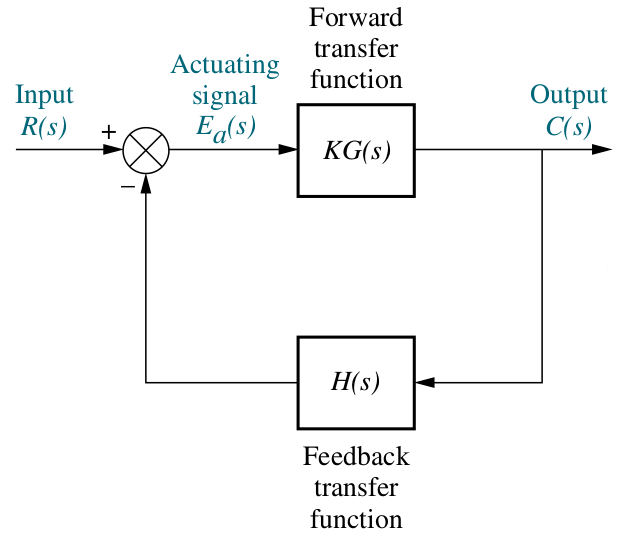
\includegraphics[width=0.5\columnwidth]{figures/Nise_Fig-8-1-a.jpg}
\end{figure}
\framebreak

Recall: 
\begin{itemize}
\item Open loop transfer function: $K \, G(s) \, H(s)$
\item Closed-loop transfer function: 
\[
T(s) \; = \; \frac{K \, G(s)}{1 + K \, G(s) \, H(s)}
\]
\end{itemize}

Margin definitions: 
\begin{itemize}
\item Gain margin $G_M$ is the factor by which we can increase $K$ before the closed-loop transfer function $T(s)$ becomes unstable. 
\item Phase margin $\phi_M$ is closedly related to the delay $T$ we can tolerate in the \linebreak sensor $H(s)$ before $T(s)$ becomes unstable. 
\begin{itemize}
\item Unfortunately the gain margin does not correspond to an intuitive concept \linebreak in the time domain. 
\end{itemize}
\end{itemize}
\framebreak

Margin evaluations: 
\begin{figure}
\centering
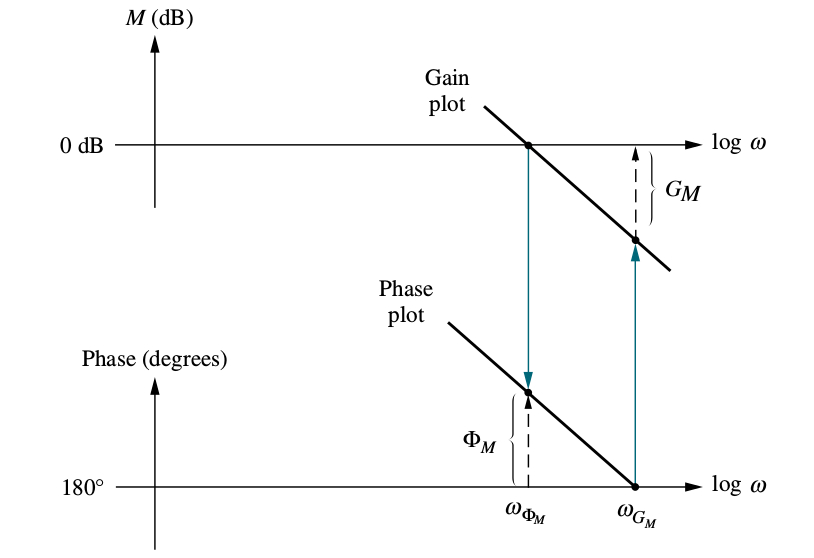
\includegraphics[width=0.68\columnwidth]{figures/Nise_Fig-10-37.jpg}
\end{figure}

\end{frame}

% =================================================================
\subsection{Phase Margin and Damping Ratio}

% -----------------------------------------------------------------
\begin{frame}[allowframebreaks]
\frametitle{\insertsection: \insertsubsection}

Recall: 
\begin{figure}
\centering
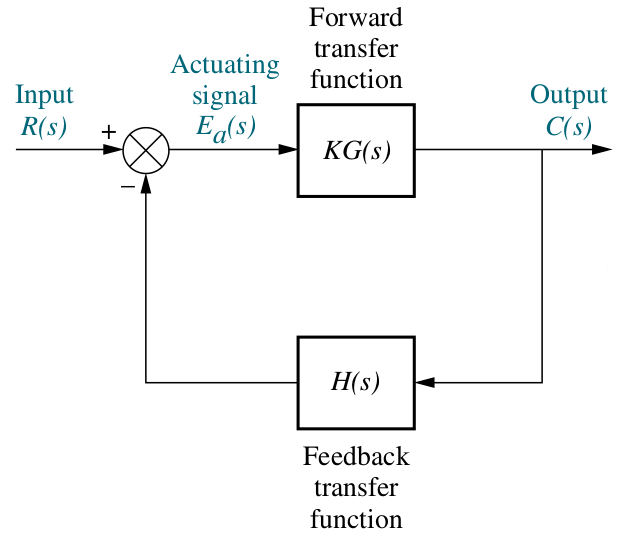
\includegraphics[width=0.5\columnwidth]{figures/Nise_Fig-8-1-a.jpg}
\end{figure}
\framebreak

Relationship between Phase Margin and Damping Ratio: 
\begin{itemize}
\item The following two quantities are related: 
\begin{itemize}
\item The phase margin $\phi_M$ of the open-loop transfer function $K \, G(s) \, H(s)$. 
\item The damping ratio $\zeta$ of the pair of dominant poles of the closed-loop \linebreak transfer function $T(s)$. 
\begin{itemize}
\item This quantity is tightly related to the percent overshoot ($\% OS$). 
\end{itemize}

\end{itemize}
\item More precisely, the relationship is: 
\[
\phi_M \; = \; \tan^{-1} \left(
\frac{2 \zeta}{ \sqrt{ -2 \zeta^2 + \sqrt{1 + 4 \zeta^4} } }
\right)
\]
\end{itemize}

\end{frame}

% -----------------------------------------------------------------
\begin{frame}[allowframebreaks]
\frametitle{\insertsection: \insertsubsection}

Using this Relationship for Design: 
\begin{enumerate}
\item Define the desired percent overshoot ($\% OS$) of the closed-loop \linebreak transfer function $T(s)$. 
\item Calculate the phase margin $\phi_M$ that the open-loop transfer function $K \, G(s) \, H(s)$ needs to have. 
\item Add lead or lag compensators to increase or decrease the phase margin \linebreak of the open-loop transfer function $K \, G(s) \, H(s)$. 
\begin{itemize}
\item While designing, strive for a compensator that achieves the desired \linebreak phase margin while minimally impacting the amplitude diagram. 
\end{itemize}

\end{enumerate}

\end{frame}

% =================================================================
\subsection{Steady-state Errors}

% -----------------------------------------------------------------
\begin{frame}[allowframebreaks]
\frametitle{\insertsection: \insertsubsection}

Recall: 
\begin{figure}
\centering
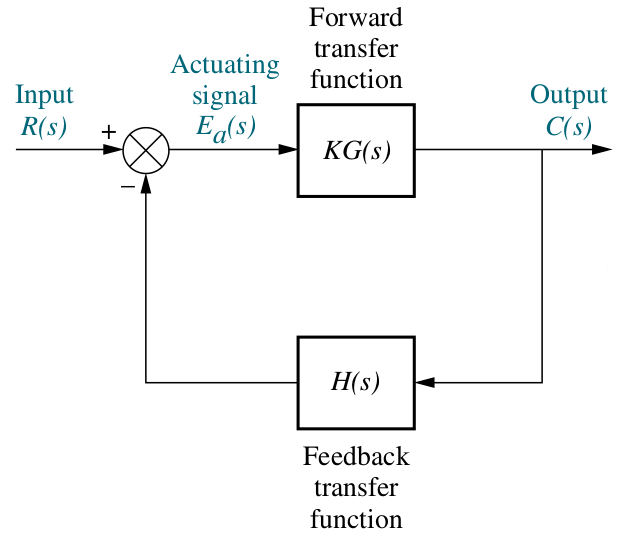
\includegraphics[width=0.5\columnwidth]{figures/Nise_Fig-8-1-a.jpg}
\end{figure}
\framebreak

Relationship between Low-frequency Asymptote and Steady-state Error: 
\begin{itemize}
\item The following two quantities are related: 
\begin{itemize}
\item The low-frequency asymptote value $M( \omega \rightarrow 0 )$ of the open-loop \linebreak transfer function $K \, G(s) \, H(s)$. 
\item The step-input error constant $K_p$ of the open-loop transfer function. 
\item The steady-state error of the closed-loop transfer function $T(s)$ when the input is a unit step, denoted $e_{step}(\infty)$. 
\end{itemize}
\item More precisely, the relationship is, in decibels: 
\[
M( \omega \rightarrow 0 ) \; = \; K_p \; = \;
\frac{1}{e_{step}(\infty)} - 1
\]
\end{itemize}
\framebreak

\begin{figure}
\centering
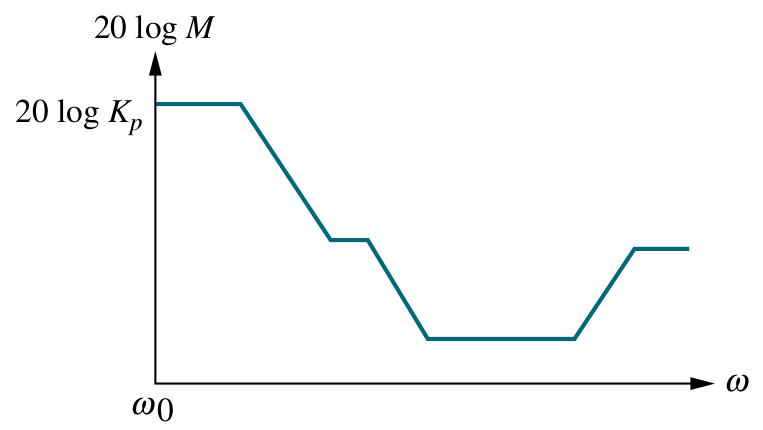
\includegraphics[width=0.6\columnwidth]{figures/Nise_Fig-10-51-a.jpg}
\end{figure}

\end{frame}

% -----------------------------------------------------------------
\begin{frame}[allowframebreaks]
\frametitle{\insertsection: \insertsubsection}

Using this Relationship for Design: 
\begin{enumerate}
\item Define the desired steady-state error of the closed-loop \linebreak transfer function $T(s)$ when the input is a unit step. 
\item Calculate the step-input error constant $K_p$ that the open-loop transfer function $K \, G(s) \, H(s)$ needs to have. 
\item Add lag or lead compensators to increase or decrease the low-frequency asymptote of the open-loop transfer function $K \, G(s) \, H(s)$. 
\begin{itemize}
\item While designing, strive for a compensator that achieves the desired \linebreak low-frequency asymptote while minimally impacting the phase diagram. 
\end{itemize}
\end{enumerate}

\end{frame}

\end{document}
